\documentclass[a4paper ,12pt]{report}
\usepackage[right=2cm, top=2cm, bottom=2.5cm, left=2cm]{geometry} 

\usepackage{amsmath}
\usepackage{mathtools}

\usepackage[ngerman, english]{babel}
\usepackage[utf8]{inputenc}

\usepackage{cite}
\usepackage[hidelinks]{hyperref}
\usepackage{url}

\usepackage{graphicx}
\graphicspath{ {../pictures/} }


\begin{document}
	\section*{Deep Q-Learning}
	The update rule of the Q-learning algorithm is given by
	\begin{equation}
	Q_{updated}(s,a) = Q(s,a) + \alpha\left[R(s,a) + \gamma \, max_{a^{\prime}} Q\left(s^{\prime}\right) - Q(s,a)\right]
	\end{equation}

	with learning rate $\alpha$, discount factor $\gamma$ and the actual reward $R(s,a)$. The action-value function $Q(a,s)$ returns the expected reward of the model choosing a specific action at a given state.
	
	Since the term $max_{a^{\prime}} Q\left(s^{\prime}\right)$ determines the action-value function of the current state, the difference of the target $Y = R(s,a) + \gamma \, max_{a^{\prime}} Q\left(s^{\prime}\right)$ and the predicted value $Q(s,a)$ describes the deviation of the momentary best choice from the prediction of the current model. The goal is to minimize this temporal difference error. This can be reached e.g. by minimizing the squared loss $(Y-Q(s,a))^2$.\cite{UBHD-68505368}
	
	\vspace{0.5cm}
	
	The state-value function $Q(s, a)$ is represented by a table with dimensions $\lvert s \lvert \times \lvert a \lvert $. Since in practise there are too many possible states to store the whole matrix or to get enough training data, the action-value function can instead be learned by regression. For function approximation we use a neural network and the error is minimized by gradient descent. \cite{Lecture}
	
	\section{Training}
	Before or while he learns to bomb crates away, the agent has to learn not to blow himself up.
	
	\newpage
	
	\section*{Notes: What we might do to improve our implementation}
	$\rightarrow$ Jetzt und/ oder Verbesserungsvorschläge in Diskussion
	
	\subsection*{Possible network adjustments}
	
	- Normierungen innerhalb des Netzes, good feature design (perceptive field figure \ref{fig:feat1}, or multiple layers for whole game field containing Walls, Bricks, Players, Danger(Bomb+Explosion), Enemies, Coins)
	
	\begin{figure}[ht]
		\caption{Feature design with perceptual field in \cite{Pommerman}}
		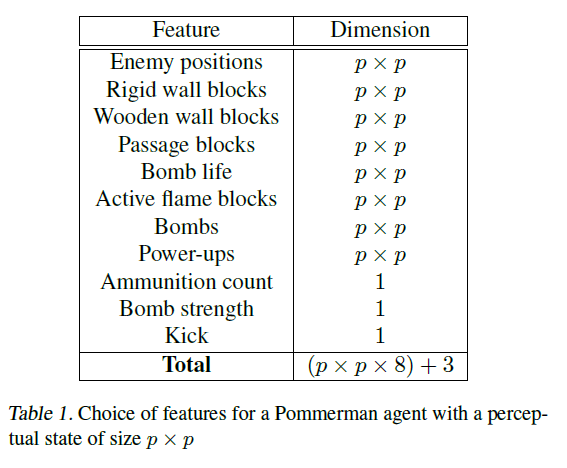
\includegraphics[width=7cm]{features_with_perceptual_field.png}
		\label{fig:feat1}
	\end{figure}
	
	- Lecture Notes: feature pre-processing via PCA
	
	- dropout algorithm; https://wandb.ai/authors/ayusht/reports/Dropout-in-PyTorch-An-Example--VmlldzoxNTgwOTE
	
	- different activation function
	
	- more layers, smaller getting layers (how others did in Figure \ref{fig:arch1} and \ref{fig:arch2})
	
	\begin{figure}[ht]
		\caption{Architecture from \cite{AlanPresentation}}
		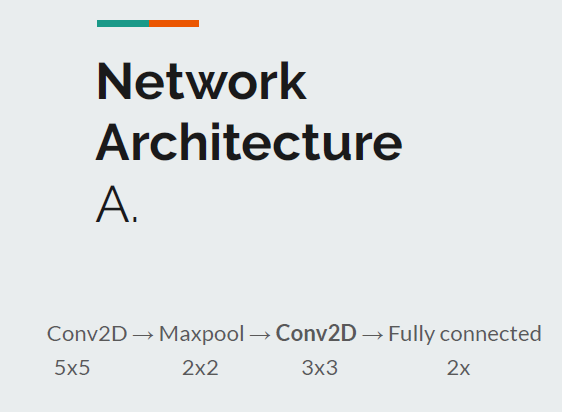
\includegraphics[width=7cm]{architecture.png}
		\label{fig:arch1}
	\end{figure}

	\begin{figure}[ht]
		\caption{Architecture from \cite{Pommerman}}
		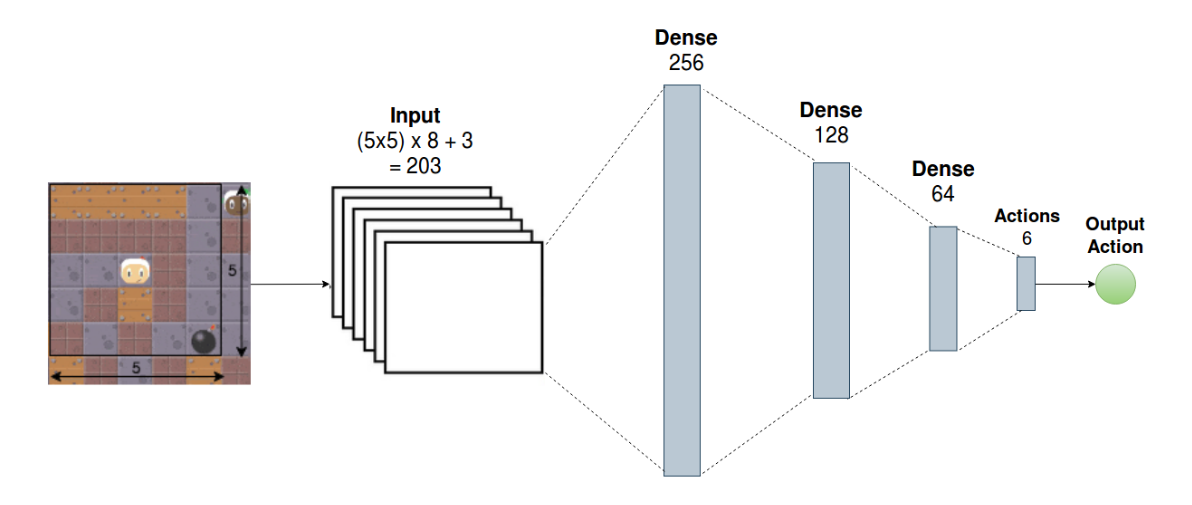
\includegraphics[width=10cm]{architecture_2.png}
		\label{fig:arch2}
	\end{figure}
	
	\subsection*{Rewards}
	
	(how others did in Figure \ref{fig:rewards}, \ref{fig:rewardsALAN})
	
	\begin{figure}[ht]
		\caption{From \cite{GoulartBomberman}}
		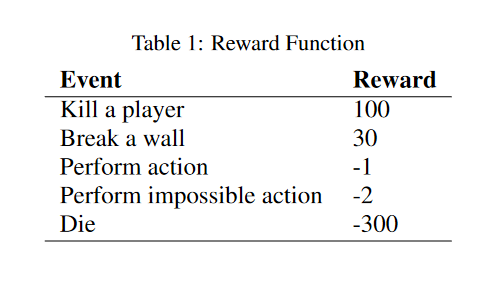
\includegraphics{rewards.png}
		\label{fig:rewards}
	\end{figure}

	\begin{figure}[ht!]
		\caption{From \cite{AlanPresentation}}
		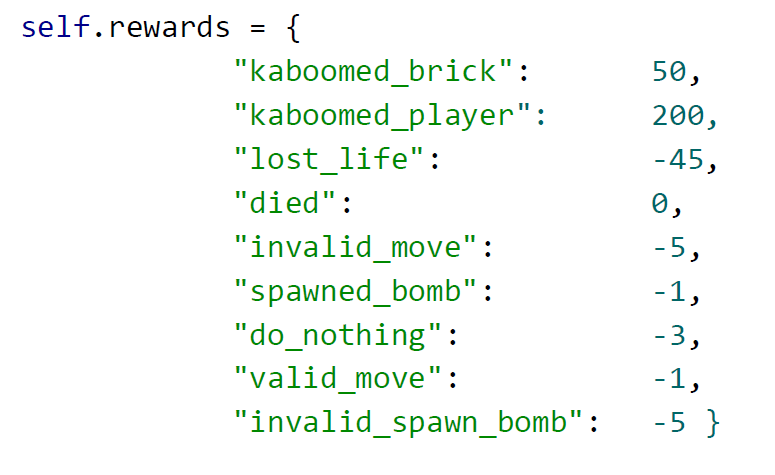
\includegraphics[width=6cm]{rewardsALAN.png}
		\label{fig:rewardsALAN}
	\end{figure}
	
	\subsection*{Reward clipping}
	"How do we assign rewards? Reward assignment varies for each game. In some games, we can assign rewards such as +1 for winning, -1 for loss, and 0 for nothing, but in some other games, we have to assign rewards such as + 100 for doing an action and +50 for doing another action. To avoid this problem, we clip all the rewards to -1 and +1." \cite{UBHD-68505368}
	
	\subsection*{Target network}
	"We are using the same Q function for calculating the target value and the predicted value. In the preceding equation, you can see the same weights  are used for both target Q and predicted Q. Since the same network is calculating the predicted value and target value, there could be a lot of divergence between these two. To avoid this problem, we use a separate network called a target network for calculating the target value." \cite{UBHD-68505368}
	
	\bibliographystyle{abbrv}
	\bibliography{bibfile}
\end{document}